\section{EXE 1 - RA}
\begin{itemize}
	\item Pulita disposizione dei record di attivazione: disposti lateralmente, per riprendere la crescita verso il basso dello stack;
	\item Eliminata la colorazione delle variabili che rappresentavano riferimento alla stessa area di memoria (quando si ha passaggio per riferimento, come nel caso della funzione \textit{f(int x, int \&y)} in cui il parametro y viene passato per riferimento);
\end{itemize}

Nella figura ~\ref{fig:ra}, si vede una visione d'insieme (parziale) della correzione dell'esercizio 1, in cui si è seguita una linea di crescita \textit{verticale}, proprio come la memoria stack: in particolare, la \textbf{crescita laterale rappresenta lo sviluppo nel tempo della memoria}, al seguirsi delle varie istruzioni.
\begin{figure}[h]
	\centering
	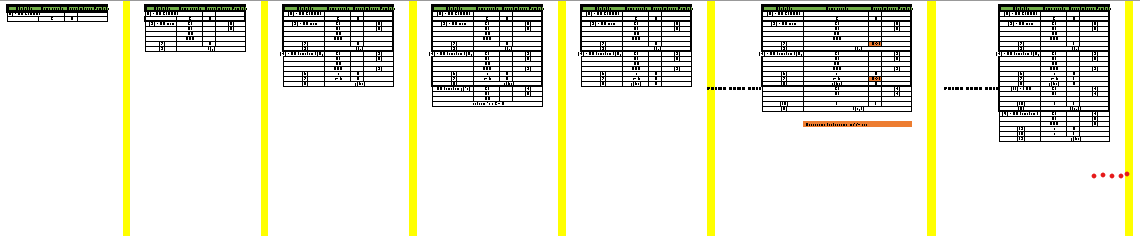
\includegraphics[width=1\textwidth]{Immagini/Partial_RA.png}
	\caption{Parziale soluzione esercizio RA}
	\label{fig:ra}
\end{figure}

\newpage
\section{EXE 2 - C}
Durante la prova, ho optato per risolvere questo esercizio per ultimo: non è stata una scelta felice, poichè sono arrivato dopo 4 ore di prova a cercare di risolvere un problema all'apparenza complicatissimo ma che, con il senno di poi, si è dimostrato risolvibile (con comunque qualche difficoltà).

\subsection{Iterativa}
Per la parte iterativa, durante la prova, non ci sono stati problemi nella stesura di una soluzione.

Nella figura ~\ref{fig:sppIt}, si vede come siamo andati a settare uno spazio di memoria dinamico, con l'istruzione \textit{malloc} di lunghezza sensata: infatti, a tutti i numeri pari da 0 a N ($N/2$) abbiamo aggiunto uno spazio necessario per aggiungere il \textit{numero terminatore} (in questo caso 1).

Il risultato poi è stato popolato con accesso tramite deferenziazione (riga 21).
\begin{figure}[h]
	\centering
	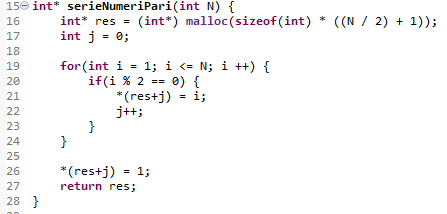
\includegraphics[width=0.6\textwidth]{Immagini/SerieNumeriPariIt.png}
	\caption{Serie numeri pari Iterativa}
	\label{fig:sppIt}
\end{figure}


\subsection{Ricorsiva senza tail}
Sicuramente questa soluzione richiedeva uno sforzo maggiore.

Riprovando a casa, sono arrivato ad una soluzione, riportata in figura ~\ref{fig:sppRecNoTail}.

\begin{figure}[h]
	\centering
	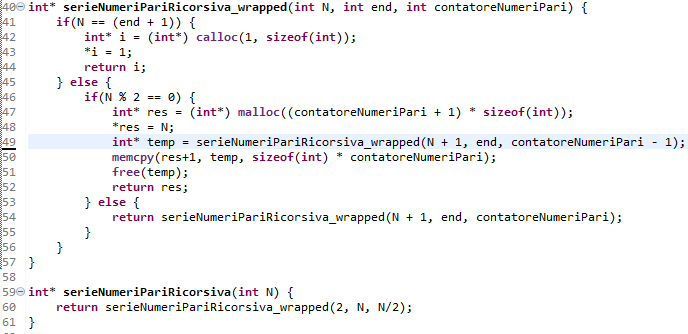
\includegraphics[width=0.6\textwidth]{Immagini/SerieNumeriPariRecNoTail.png}
	\caption{Serie numeri pari ricorsiva senza tail [operazioni di debug omesse]]}
	\label{fig:sppRecNoTail}
\end{figure}

\begin{figure}[h]
	\centering
	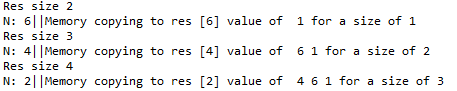
\includegraphics[width=0.6\textwidth]{Immagini/SerieNumeriPariRecNoTailDebug.png}
	\caption{Serie numeri pari ricorsiva senza tail - debug print}
	\label{fig:sppRecNoTailLog}
\end{figure}

Rispetto alla prova, ho apportato questi cambiamenti:
\begin{itemize}
	\item Ho inserito una funzione wrapper, per nascondere all'utente il fatto che la scansione dei numeri parta da 2 (ho scartato lo 0 e l'1 che sono dispari) arrivando fino a N, così da ritornare un risultato che sia in ordine crescente;
	\item \textit{contatoreNumeriPari} è utilizzato per poter sfruttare al meglio il comando di memcpy, in maniera tale da copiare/allocare solamente la quantità di memoria necessaria
	\item Il risultato è salvato in una variabile temporanea per poterne poi fare il free: questo fa si che i valori numerici vengano ananlizzati in maniera decrescente (prima annido le chiamate per valori decrescenti, e poi analizzo i risultati in maniera decrescente)
	\item La condizione d'uscita si ha quando raggiungo il valore successivo al valore passato in input dall'utente (end + 1);
	\item Essendo che salvo il risultato in una variabile temporanea (riga 49), per poterne poi fare il free, l'analisi dei risultati sarà effettuato in ordine inverso: è per questo motivo che il contatore dei numeri pari parte dal valore completo (N/2) e decresce (e quindi i valori da copiare dovranno essere 1, e via via crescenti);
\end{itemize}

\subsection{Ricorsiva CON tail}
La versione tail è stata leggermente modificata: anche qui, come nella versione non tail, ho inserito una funzione wrapper, per nascondere all'utente il comportamento a basso livello della funzione.

Nello specifico anche qui faccio partire il conteggio daa 2, per farlo concludere quando raggiunge il valore (end + 1).

\section{EXE 3 - C++ distruttore}
Il distruttore è il metodo duale del costruttore: esso serve principalmente ad eliminare gli oggetti
della memoria, andando quindi a liberare spazio in memoria.

Il distruttore viene chiamato automaticamente dal compliatore quando la variabile esce dal suo scope.
Questa eliminazione automatica però non avviene per i puntatori: quindi se ho un puntatore (allocato tramite la funzione malloc) sarà necessario che sia invocato esplicitamenteun comando di free per evitare un memory leakage.

Nel caso di utilizzi di sottoclassi è sempre meglio dichiarare il distruttore virtual così che chiami tutti i distruttori delle superclassi (dalla sottoclasse e poi fino alla superclasse)
\section{EXE 4 - Opachi}

Rispetto alla soluzione proposta in prova, sono andato a snellire il metodo \textit{somma} utilizzando l'init \textit{make} come si vede in figura ~\ref{fig:makeSomma}.

\begin{figure}[h]
	\centering
	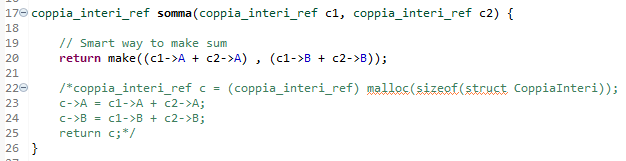
\includegraphics[width=0.6\textwidth]{Immagini/makeSommaOpachi.png}
	\caption{Metodo \textit{make}}
	\label{fig:makeSomma}
\end{figure}

\section{EXE 5 - Visitor}
Durante la prova avevo inserito anche il Visitor anche per le \textit{FigureGeometriche} astratte: questo perchè nel metodo \textit{calcolaMax} andavo a chiamare la funzione \textit{visit} invece che \textit{accept}, il chè quindi mi ha portato ad inserire il visitor anche per la classe astratta.

Ho corretto quindi il metodo \textit{calcolaMax} come si vede in figura ~\ref{fig:calcolaMax}.

\begin{figure}[h]
	\centering
	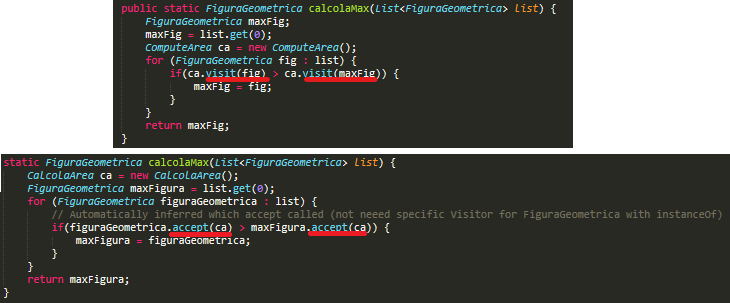
\includegraphics[width=0.6\textwidth]{Immagini/calcolaMax.png}
	\caption{Confronto tra metodi calcolaMax (prova sopra e correzione sotto)}
	\label{fig:calcolaMax}
\end{figure}

\section{EXE 6 - Scala}
Nella correzione della prova di Scala sono andata ad inserire il wrapper, come si vede in figura ~\ref{fig:scalaWrap}: ho sfruttato la possibilità che Scala offre di definire funzioni \textit{inline}.

\begin{figure}[h]
	\centering
	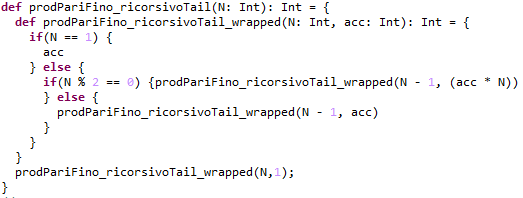
\includegraphics[width=0.6\textwidth]{Immagini/scalaWrap.png}
	\caption{Wrap in Scala}
	\label{fig:scalaWrap}
\end{figure}

Ho inoltre anche aggiunto l'utilizzo delle \textit{High Order Functions}: nella specifico ho inserito una \textit{HOF} per andare a generalizzare il criterio della funzione: nello specifico, con questa \textit{HOF} si può andare a settare il valore per cui poi sommeremo solamente i numeri divisibili per tale valore.

Per esempio, nel main di prova, ho settato il criterio pari a 5: in questo modo sommeremo tutti i numeri divisibili per 5.